%iffalse
\let\negmedspace\undefined
\let\negthickspace\undefined
\documentclass[journal,,12pt,onecolumn]{IEEEtran}
\usepackage{cite}
\usepackage{amsmath,amssymb,amsfonts,amsthm}
\usepackage{algorithmic}
\usepackage{graphicx}
\usepackage{textcomp}
\usepackage{xcolor}
\usepackage{txfonts}
\usepackage{listings}
\usepackage{enumitem}
\usepackage{mathtools}
\usepackage{gensymb}
\usepackage{comment}
\usepackage[breaklinks=true]{hyperref}
\usepackage{tkz-euclide} 
\usepackage{listings}
\usepackage{gvv}                                        
%\def\inputGnumericTable{}                                 
\usepackage[latin1]{inputenc}                                
\usepackage{color}                                            
\usepackage{array}                                            
\usepackage{longtable}                                       
\usepackage{calc}                                             
\usepackage{multirow}                                         
\usepackage{hhline}                                           
\usepackage{ifthen}                                           
\usepackage{lscape}
\usepackage{tabularx}
\usepackage{array}
\usepackage{float}
\usepackage{tikz}
\usepackage{multicol}



\newtheorem{theorem}{Theorem}[section]
\newtheorem{problem}{Problem}
\newtheorem{proposition}{Proposition}[section]
\newtheorem{lemma}{Lemma}[section]
\newtheorem{corollary}[theorem]{Corollary}
\newtheorem{example}{Example}[section]
\newtheorem{definition}[problem]{Definition}
\newcommand{\BEQA}{\begin{eqnarray}}
\newcommand{\EEQA}{\end{eqnarray}}
\newcommand{\define}{\stackrel{\triangle}{=}}
\theoremstyle{remark}
\newtheorem{rem}{Remark}

% Marks the beginning of the document
\begin{document}
\bibliographystyle{IEEEtran}
\vspace{3cm}

\title{EE\\2007}
\author{EE24BTECH11063 - Y.Harsha Vardhan Reddy}
\maketitle

\bigskip

\renewcommand{\thefigure}{\theenumi}
\renewcommand{\thetable}{\theenumi}

\section*{Q.1-Q.20 carry one mark each}

\begin{enumerate}
    \item A single phase full-wave half-controlled bridge converter feeds an inductive load. The two SCRs in the converter are connected to a common DC bus. The converter has to have a freewheeling diode 
    \begin{enumerate}
            \item because the converter inherently does not provide for free-wheeling
            \item because the converter does not provide for free-wheeling for high values of triggering angles
             \item or else the free-wheeling action of the converter will cause shorting of the AC supply
            \item or else if a gate pulse  to one of the SCRs is missed, it will subsequently cause a high load current in the other SCR
    \end{enumerate}
    \bigskip
\item The electromagnetic torque $T_c$ of a drive, and its connected load torque $T_L$ are as shown below. Out of the operating points A,B,C and D, the stable ones are
\begin{figure}[H]
   \centering
   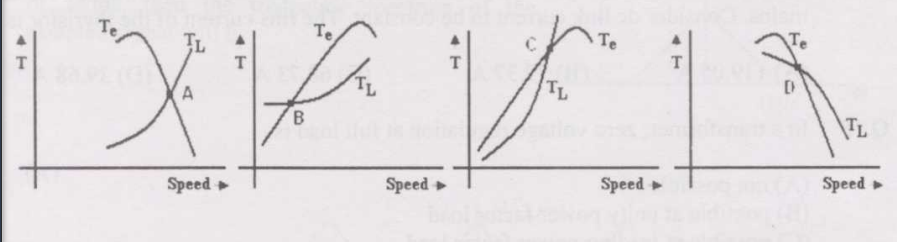
\includegraphics[width=0.7\linewidth]{figs/fig_1.png}
   \label{stemplot}
\end{figure}
\begin{enumerate}
    \begin{multicols}{4}
        \item A,C,D
        \item B,C
        \item A,D
        \item B,C,D
    \end{multicols}
\end{enumerate}
\bigskip
\item "Six MOSFETs connected in a bridge configuration (having no other power device) MUST be operated as a Voltage Source Inverter(VSI)". This statement is
\begin{enumerate}
    \item True, because being majority carier devices, MOSFETs are voltage driven
    \item True, because MOSFETs have inherently anti-parallel diodes 
    \item False, because it can be operand both as Current Source Inverter(CSI) or a VSI
    \item False, because MOSFETs can be operated as excellent constant current sources in the saturation region
\section*{Q.21 to Q.75 carry two marks each.}
\end{enumerate}
\bigskip
\item The input signal $V_{in}$ shown in the figure is a 1kHz square wave voltage that alternates between +7V and -7V with a 50\% duty cycle. Both transistors have the same current gain, which is large. The circuit delivers power to the load resistor $R_L$. What is the efficiency of this circuit for the given input? Choose the closest answer
\begin{figure}[H]
   \centering
   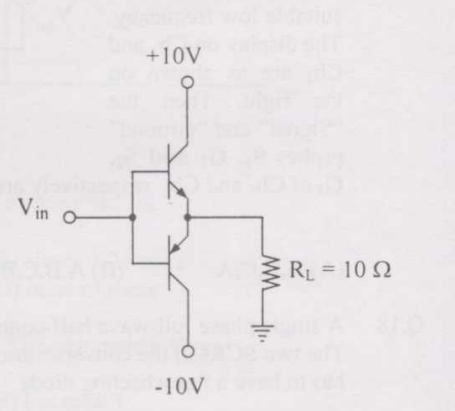
\includegraphics[width=0.7\linewidth]{figs/fig_2.png}
   \label{stemplot}
\end{figure}

\begin{enumerate}
    \begin{multicols}{4}
        \item 46\%
        \item 55\%
        \item 63\%
        \item 92\%
    \end{multicols}
\end{enumerate}
\bigskip
\item A,B,C and D are input bits, and Y is the output bit in the XOR gate circuit of the figure below. Which of the following statements about the sum S of A,B,C,D and Y is correct?
\begin{figure}[H]
   \centering
   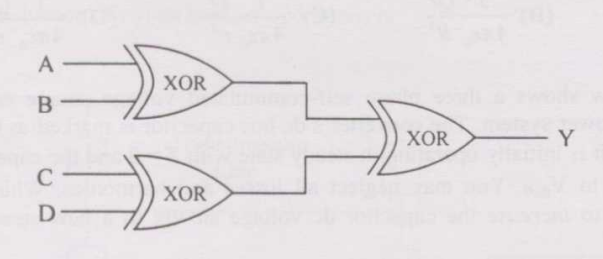
\includegraphics[width=0.7\linewidth]{figs/fig_3.png}
   \label{stemplot}
\end{figure}
\begin{enumerate}
        \item S is always either zero or odd
        \item S is always either zero or even
        \item S = 1 only if the sum of A,B,C and D is even 
        \item S = 1 only if the sum of A,B,C and D is odd
\end{enumerate}
\bigskip
\item The differential equation $\frac{dx}{dt}=\frac{1-x}{\tau}$ is discretised using Euler's numerical integration method with a time step $\Delta T > 0$. What is the maximum permissible value of $\Delta T$ to ensure stability of the solution of the corresponding discrete time equation?

\begin{enumerate}
    \begin{multicols}{4}
        \item 1
        \item $\frac{\tau}{2}$
        \item $\tau$
        \item $2\tau$
    \end{multicols}
\end{enumerate}
\bigskip
\item The switch S in the circuit of the figure is initially closed. It is opened at time t=0. You may neglect the Zener diode forward voltage drops. What is the behaviour of $V_{OUT}$ for $t>0$? 
\begin{figure}[H]
   \centering
   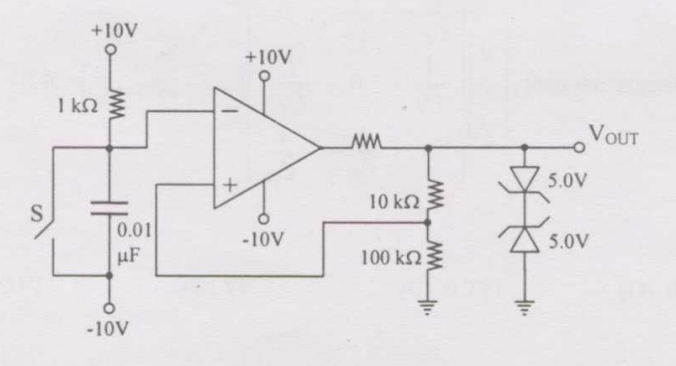
\includegraphics[width=0.7\linewidth]{figs/fig_4.png}
   \label{stemplot}
\end{figure}
\begin{enumerate}
    \item It makes a transition from -5V to +5V at $t=12.98\mu s$
    \item It makes a transition from -5V to +5V at $t=2.57\mu s$
    \item It makes a transition from +5V to -5V at $t=12.98\mu s$
    \item It makes a transition from +5V to -5V at $t=2.57\mu s$

\end{enumerate}
\bigskip
\item A solid sphere made of insulating material has a radius R and has a total charge $Q$ distributed uniformly in its volume. What is the magnitude of the electric field intensity, E, at a distance $r\brak{0<r<R}$ inside the sphere?
\begin{enumerate}
    \begin{multicols}{4}
        \item $\frac{1}{4\pi\epsilon_0}\frac{Qr}{R^3}$
        \item $\frac{3}{4\pi\epsilon_0}\frac{Qr}{R^3}$
        \item $\frac{1}{4\pi\epsilon_0}\frac{Q}{r^2}$
        \item $\frac{1}{4\pi\epsilon_0}\frac{QR}{r^3}$
    \end{multicols}
\end{enumerate}
\bigskip
\item The figure below shows a three phase self-commutated voltage source converter connected to a power system. The converter's dc bus capacitor is marked as C in the figure. The converter's dc bus capacitor is marked as C in the figure. The circuit is initially operating in steady state with $\delta=0$ and the capacitor dc voltage is equal to $V_{dc0}$. You may neglect all losses and harmonics. What action should be taken to increase the capacitor dc voltage slowly to a new steady state value?
\begin{figure}[H]
   \centering
   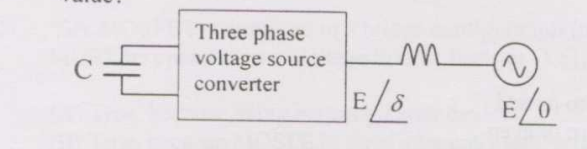
\includegraphics[width=0.7\linewidth]{figs/fig_5.png}
   \label{stemplot}
\end{figure}
\begin{enumerate}
        \item Make $\delta$ positive and maintain it at a positive value
        \item Make $\delta$ positive and return it to its original value
        \item Make $\delta$ negative and maintain it at a negative value
        \item Make $\delta$ negative and return it to its original value
\end{enumerate}
\bigskip
\item The total reactance and total susceptance of a lossless overhead EHV line, operating at 50Hz, are given by 0.045 pu and 1.2 pu respectively. If the velocity of wave propagation is $3 \times 10^5$ km/s, then the approximate length of the line is
\begin{enumerate}
    \begin{multicols}{4}
        \item 122 km
        \item 172 km
        \item 222 km
        \item 272 km
    \end{multicols}
\end{enumerate}
\bigskip
\item Consider the protection system shown in the figure below. The circuit breakers, numbered from 1 to 7 are of identical type. A single line to ground fault with zero fault impedance occurs at the midpoint of the line (at point F), but circuit breaker 4 fails to operate ("stuck breaker"). If the relays are coordinated correctly, a valid sequence of circuit breaker operations is
\begin{figure}[H]
   \centering
   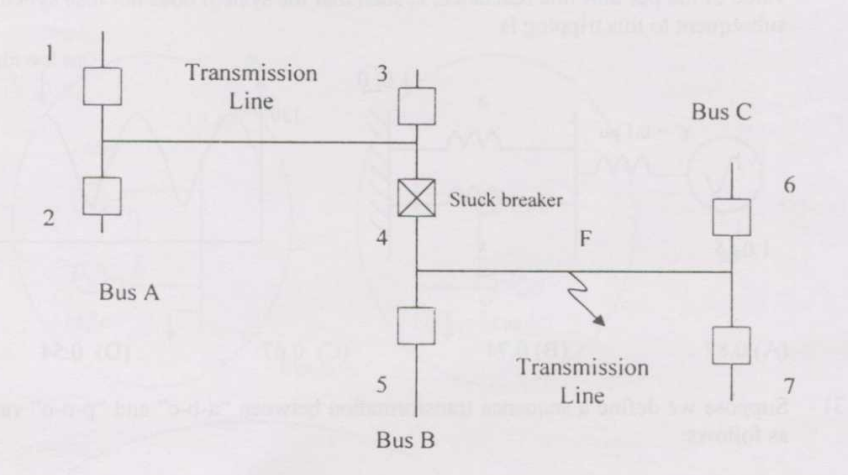
\includegraphics[width=0.7\linewidth]{figs/fig_6.png}
   \label{stemplot}
\end{figure}
\begin{enumerate}
    \begin{multicols}{4}
        \item 1,2,6,7,3,5
        \item 1,2,5,6,7,3
        \item 5,6,7,3,1,2
        \item 5,1,2,3,6,7
    \end{multicols}
\end{enumerate}
\bigskip
\item A three phase balanced star connected voltage source with frequency $\omega$ rad/s is connected to a star balanced load which is purely inductive. The instantaneous line currents and phase to neutral voltages are denoted by $\brak{i_a,i_b,i_c}$ and $\brak{v_{an},v_{bn},v_{cn}}$ respectively, and their rms values are denoted by V and I.
\begin{align*}
    \text{If }R=\myvec{v_{an}&v_{bn}&v_{cn}}\myvec{0&\frac{1}{\sqrt{3}}&-\frac{1}{\sqrt{3}}\\
    -\frac{1}{\sqrt{3}}&0&\frac{1}{\sqrt{3}}\\
    \frac{1}{\sqrt{3}}&-\frac{1}{\sqrt{3}}&0}\myvec{i_a\\i_b\\i_c},
\end{align*}
then the magnitude of R is
\begin{enumerate}
    \begin{multicols}{4}
        \item 3VI
        \item VI
        \item 0.7VI
        \item 0
    \end{multicols}
\end{enumerate}
\bigskip
\item Consider a synchronous generator connected to an infinite bus by two identical parallel transmission lines. The transient reactance $x'$ of the generator is 0.1 pu and the mechanical power input to it is constant at 1.0 pu. Due to some previous disturbance, the rotor angle $\brak{\delta}$ is undergoing an undamped oscillation, with the maximum value of $\delta\brak{t}$ equal to $130\degree$. One of the parallel lines trips due to relay maloperation at an instant when $\delta\brak{t}=130\degree$ as shown in the figure. The maximum value of the per unit line reactance, x, such that the system does not lose synchronism subsequent to this tripping is
\begin{figure}[H]
   \centering
   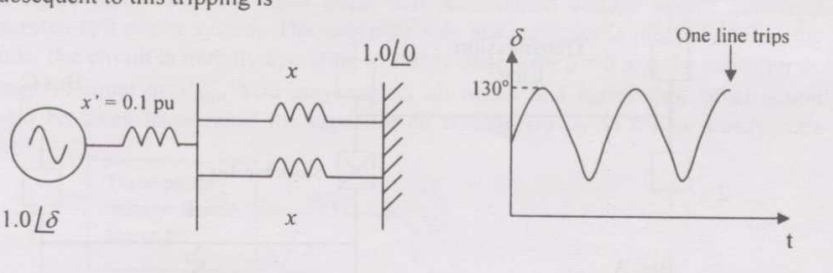
\includegraphics[width=0.7\linewidth]{figs/fig_7.png}
   \label{stemplot}
\end{figure}
\begin{enumerate}
  \begin{multicols}{4}
        \item 0.87
        \item 0.74
        \item 0.67
        \item 0.54
    \end{multicols}
\end{enumerate}
\bigskip
\item Suppose we define a sequence transformation between $"a-b-c"$ and $"p-n-o"$ variables as follows:
\begin{align*}
    \myvec{f_a\\f_b\\f_c}=k\myvec{1&1&1\\{\alpha}^2&\alpha&1\\\alpha&{\alpha}^2&1}\myvec{f_p\\f_n\\f_o}\text{ where} \alpha=e^{j\frac{2\pi}{3}} \text{ and k is a constant}
\end{align*}
Now ,if it is given that: $\myvec{V_p\\V_n\\V_p}=\myvec{0.5&0&0\\0&0.5&0\\0&0&2.0}\myvec{i_p\\i_n\\i_o}$ and $\myvec{V_a\\V_b\\V_c}=Z\myvec{i_a\\i_b\\i_c}$ then, 
\begin{enumerate}
    \begin{multicols}{2}
        \item $Z=\myvec{1.0&0.5&0.75\\0.75&1.0&0.5\\0.5&0.75&1.0}$
        \columnbreak
        \item $Z=\myvec{1.0&0.5&0.5\\0.5&1.0&0.5\\0.5&0.5&1.0}$
        \end{multicols}
        \begin{multicols}{2}
        \item $Z=\myvec{1.0&0.75&0.5\\0.5&1.0&0.75\\0.75&0.5&1.0}$
        \item $Z=\frac{k^2}{3}\myvec{1.0&-0.5&-0.5\\-0.5&1.0&-0.5\\-0.5&-0.5&1.0}$
    \end{multicols}
\end{enumerate}
\bigskip
\item Consider the two power systems shown in figure A below, which are initially not interconnected, and are operating in steady state at the same frequency. Separate loadflow solutions are computed individually for the two systems, corresponding to this scenario. The bus voltage phasors so obtained are indicated on figure A. These two isolated systems are now interconnected by a short transmission line as shown in figure B, and it is  found that $P_1=P_2=Q_1=Q_2=0$.
\begin{figure}[H]
   \centering
   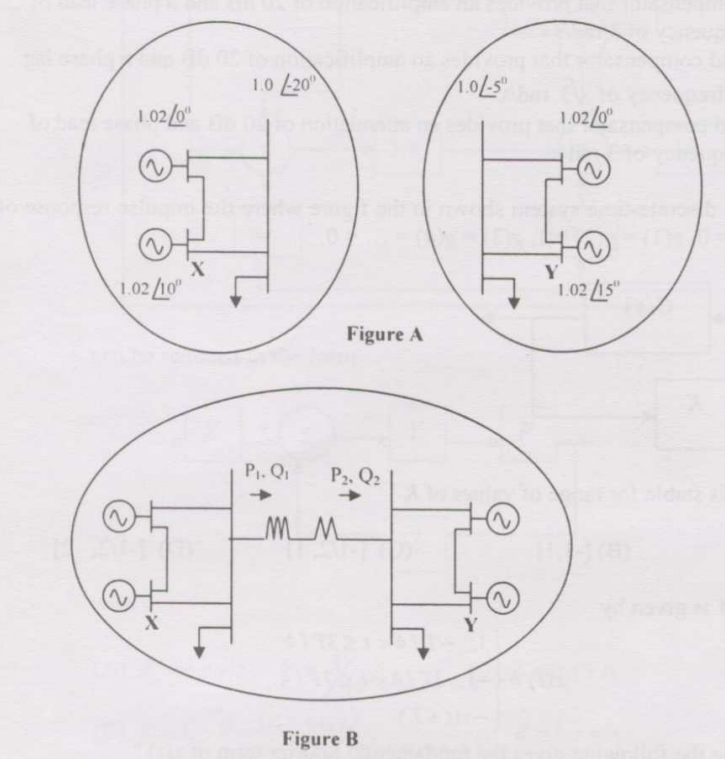
\includegraphics[width=0.7\linewidth]{figs/fig_8.png}
   \label{stemplot}
\end{figure}
The bus voltage phase angular difference between generator bus X and generator bus Y after the interconnection is
\begin{enumerate}
    \begin{multicols}{4}
        \item $10^0$
        \item $25^0$
        \item $-30^0$
        \item $30^0$
    \end{multicols}
\end{enumerate}
\bigskip
\item The octal equivalent of the HEX number \textbf{AB.CD} is
\begin{enumerate}
    \begin{multicols}{4}
        \item 253.314
        \item 253.632
        \item 526.314
        \item 526.632
    \end{multicols}
\end{enumerate}
\bigskip
\item If $x=Re\;G\brak{j\omega}$, and $y=Im\;G\brak{j\omega}$ then for $\omega \to 0^+$, the Nyquist plot for $G\brak{s}=\frac{1}{s\brak{s+1}\brak{s+2}}$ becomes asymptotic to the line 
\begin{enumerate}
    \begin{multicols}{4}
        \item $x=0$
        \item $x=-\frac{3}{4}$
        \item $x=y-\frac{1}{6}$
        \item $x=\frac{y}{\sqrt{3}}$
    \end{multicols}
\end{enumerate}
\end{enumerate}
\end{document}
